Den heutigen Projektablauf bei der allink könnte man am Besten als ``natürliches Vorgehen''
umschreiben. Ein potentielles Projekt kommt an einen Partner heran, entweder über 
eine Anfrage oder eine Akquisition, der spricht sich mit den anderen Partner ab 
und nimmt dann die Mitarbeiter mit in das Projekt, die er als nötig erachtet.
Dies kommt einem Projektmanamgement organisiert über die Linie am nächsten.

Der Projektablauf wird in drei Prozesse, die Projektannahme und Offertenerstellung,
die Projektdurchführung und der Projektabschluss unterteilt und dazu die 
Ablaufdiagramme erstellt. Darin wird jede Aktion mit einer eindeutigen Nummer versehen,
um danach darauf im beschreibenden Text verweisen zu können. Nach einer Entscheidung erhöht
sich die Laufnummer jeweils um eine ganze Zahl, um die verschiedenen Wege hervorzuheben.
Zusätzlich werden die Abläufe um die Tools, die verwendet werden, ergänzt.
Es werden nicht immer alle erwähnten Tools in dem selben Projekt eingesetzt,
jedoch Projektübergreifend betrachtet, kommen alle mal beim zugeordneten Schritt 
zum Einsatz. Die verwendete Software wird zu einem späteren Zeitpunkt separat
behandelt, da es zu diesem Zeitpunkt das ``Wie?'' und nicht ``Womit?'' betrachtet
wird.

\subsection{Projektannahme und Offertenerstellung}
In der nachfolgenden Darstellungen \ref{pic:01_ist_prozesse_offerte_01} und
\ref{pic:01_ist_prozesse_offerte_02} ist der aktuelle Prozess der Offertenerstellung 
ersichtlich. Die darin verwickelten Akteuere sind der Kunde und der bzw. die Partner.
Eine Projektanfrage endet entweder in einer Absage oder einem Start eines neuen 
Projektes. Wenn das Projekt nicht zustande kommt, werden zurzeit die Aufwände der
Akquisition und der Offertenerstellung vernachlässigt und somit von
den durchgeführten Projekten getragen.

\begin{figure}[htbp]
\begin{center}
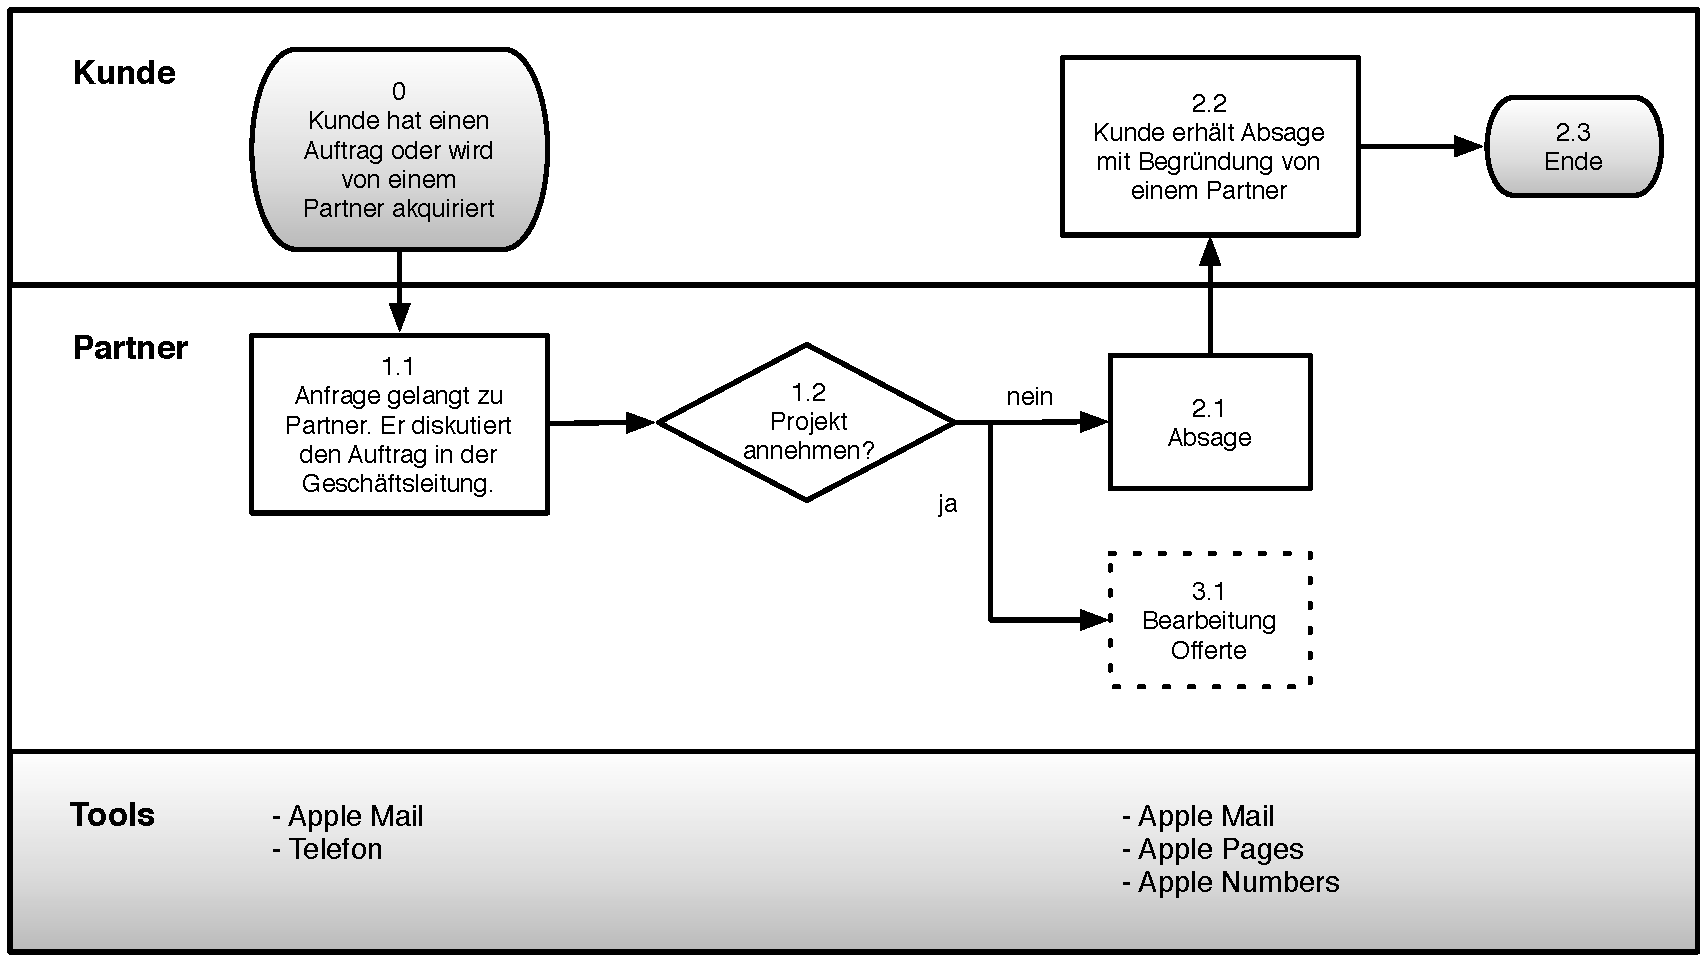
\includegraphics[width=0.99\textwidth,angle=0]{./bilder/analyse/01_ist_prozesse_offerte_01.pdf}
\caption{Offertenerstellungs Prozess von allink März 2011 1/2}
\label{pic:01_ist_prozesse_offerte_01}
\end{center}
\end{figure}

Als Start eines Projektablaufes wird entweder ein neues Projekt akquiriert, 
durch eine direkte Anfrage an ein Unternehmen oder einen Pitch\footnote{Als Pitch 
wird der Wettbewerb zwischen verschiedenen Agenturen um einen Auftrag eines 
Unternehmens bezeichnet.}, oder die Anfrage kommt direkt von einem Kunden (\textbf{0}). 
Die Projekte gelangen zum heutigen Zeitpunkt immer als erstes zu einem Partner. 
Sehr selten bringt ein Mitarbeiter durch einen seiner Kontakte ein Projekt ein. 
Aber auch in diesem Fall, würde es als erstes an einen Partner herangetragen.
Dieser diskutiert den möglichen Auftrag mit den anderen Partnern in der 
Geschäftsleitung (\textbf{1.1}). Diese entscheide demokratisch ob ein Projekt 
angenommen oder abgelehnt wird (\textbf{1.2}). Sofern nicht alle Partner anwesend 
sein können, haben die anderen Partner die Kompetenz, alleine zu entscheiden.

Im Falle einer Absage (\textbf{2.1}) tritt ein Partner wieder mit dem Kunden in Kontakt.
In den meisten Fällen natürlich der Partner, der bereits mit dem Kunden Kontakt
hatte. Dem Kunden wird erklärt, aus welchen Gründen das Projekt nicht angenommen
und durchgeführt werden kann (\textbf{2.2}).

\begin{figure}[htbp]
\begin{center}
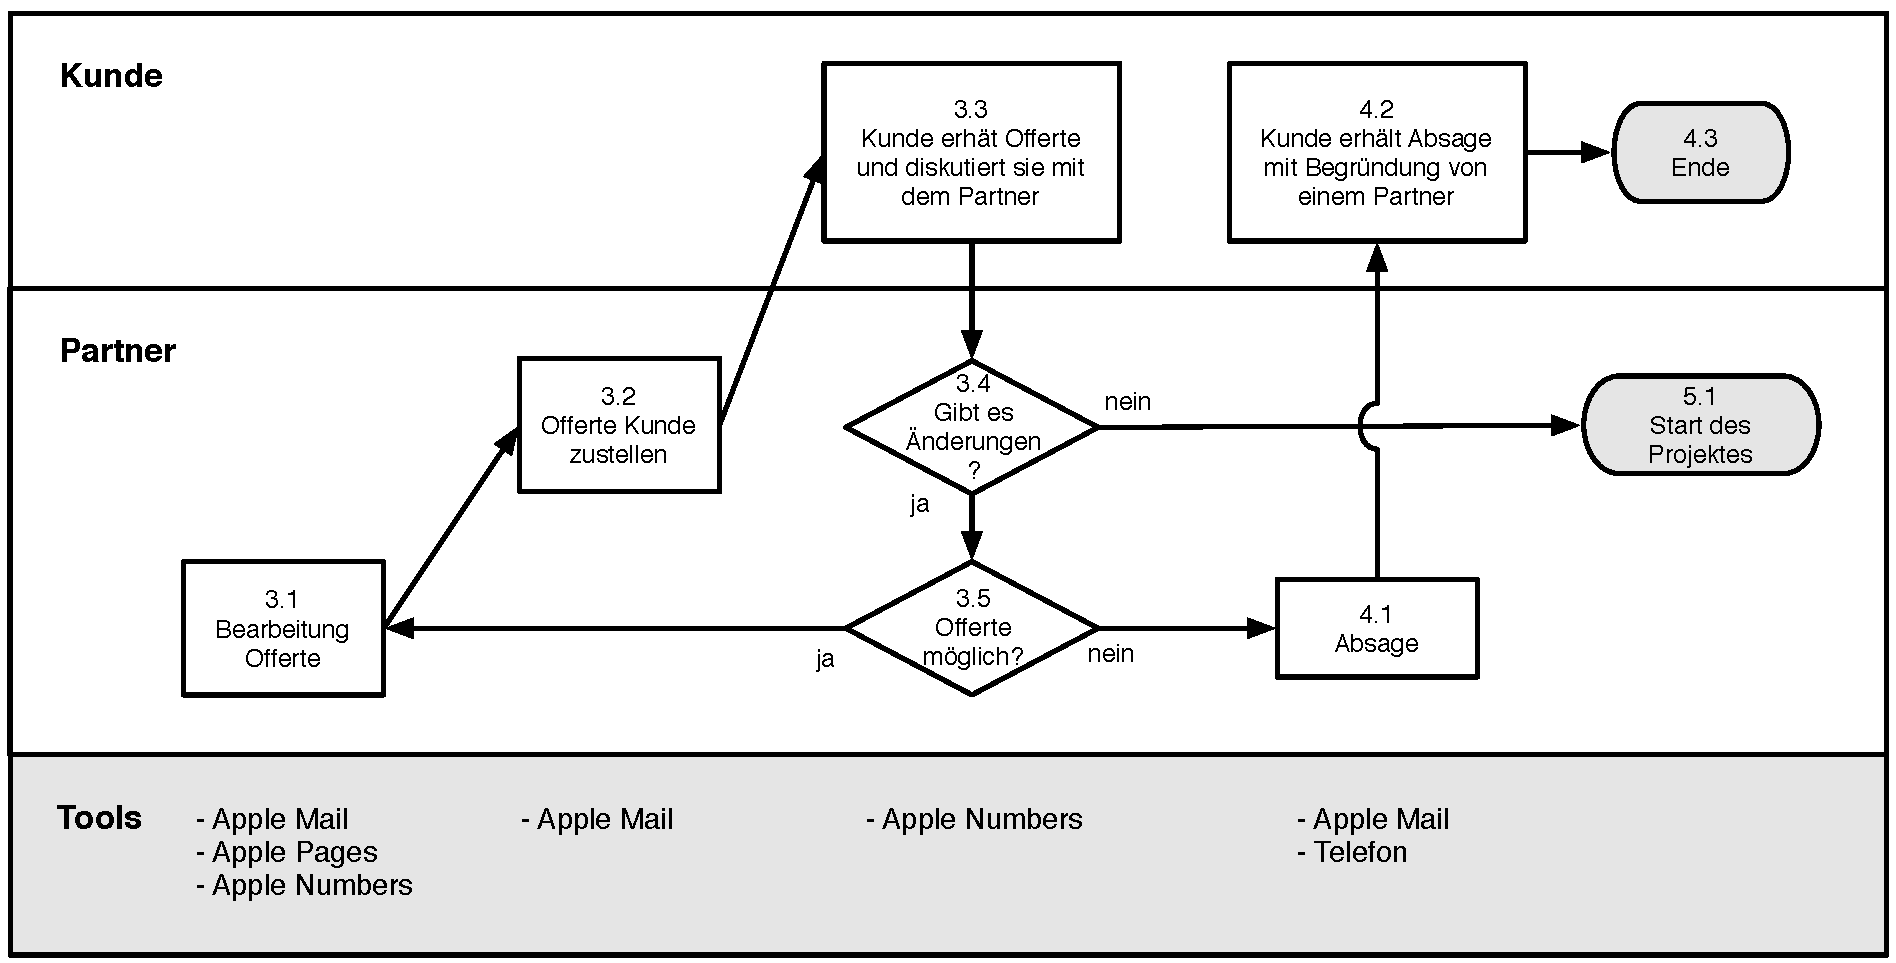
\includegraphics[width=0.99\textwidth,angle=0]{./bilder/analyse/01_ist_prozesse_offerte_02.pdf}
\caption{Offertenerstellungs Prozess von allink März 2011 2/2}
\label{pic:01_ist_prozesse_offerte_02}
\end{center}
\end{figure}

Sollte das Projekt angenommen werden, wird auf Grund den zu erbringenden
Dienstleistungen eine möglichst genaue Offerte erstellt (\textbf{3.1}). Diese Schätzungen
basieren überwiegend auf Erfahrungswerten aus anderen Projekten.
Die Offerte wird dann dem Kunden zugestellt (\textbf{3.2}). In vielen Fällen wird dem Kunden
die Offerte präsentiert und genauer erklärt.
Der Kunde diskutiert dann mit dem oder den Partnern die Offerte (\textbf{3.3}) und bringt
bei bedarf Änderungen und Wünsche an.
Kann man sich mit dem Kunden nicht einigen, also wünscht der Kunde Änderungen
an der Offerte oder den zu erbringenden Dienstleistungen (\textbf{3.4}), die von unserer Seite
nicht mehr möglich sind (\textbf{3.5}), muss das Projekt abgesagt werden (\textbf{4.1}).
Dem Kunden wird erklärt, aus welchen Gründen die Offerte nicht angepasst oder
die Dienstleistung nicht erbracht werden kann (\textbf{4.2}).

Im Falle einer Einigung und einer Auftragserteilung startet das eigentliche
Projekt (\textbf{5.1}).

\clearpage

\subsection{Projektdurchführung}
In der ersten Phase der Projektdurchführung sammelt der Projektleiter bzw.
Partner alle nötigen Informationen, die zur Bearbeitung des Projektes notwendig sind.
Danach erstellt er Arbeitspakete, die er wiederum an die Mitarbeiter verteilt.

\begin{figure}[htbp]
\begin{center}
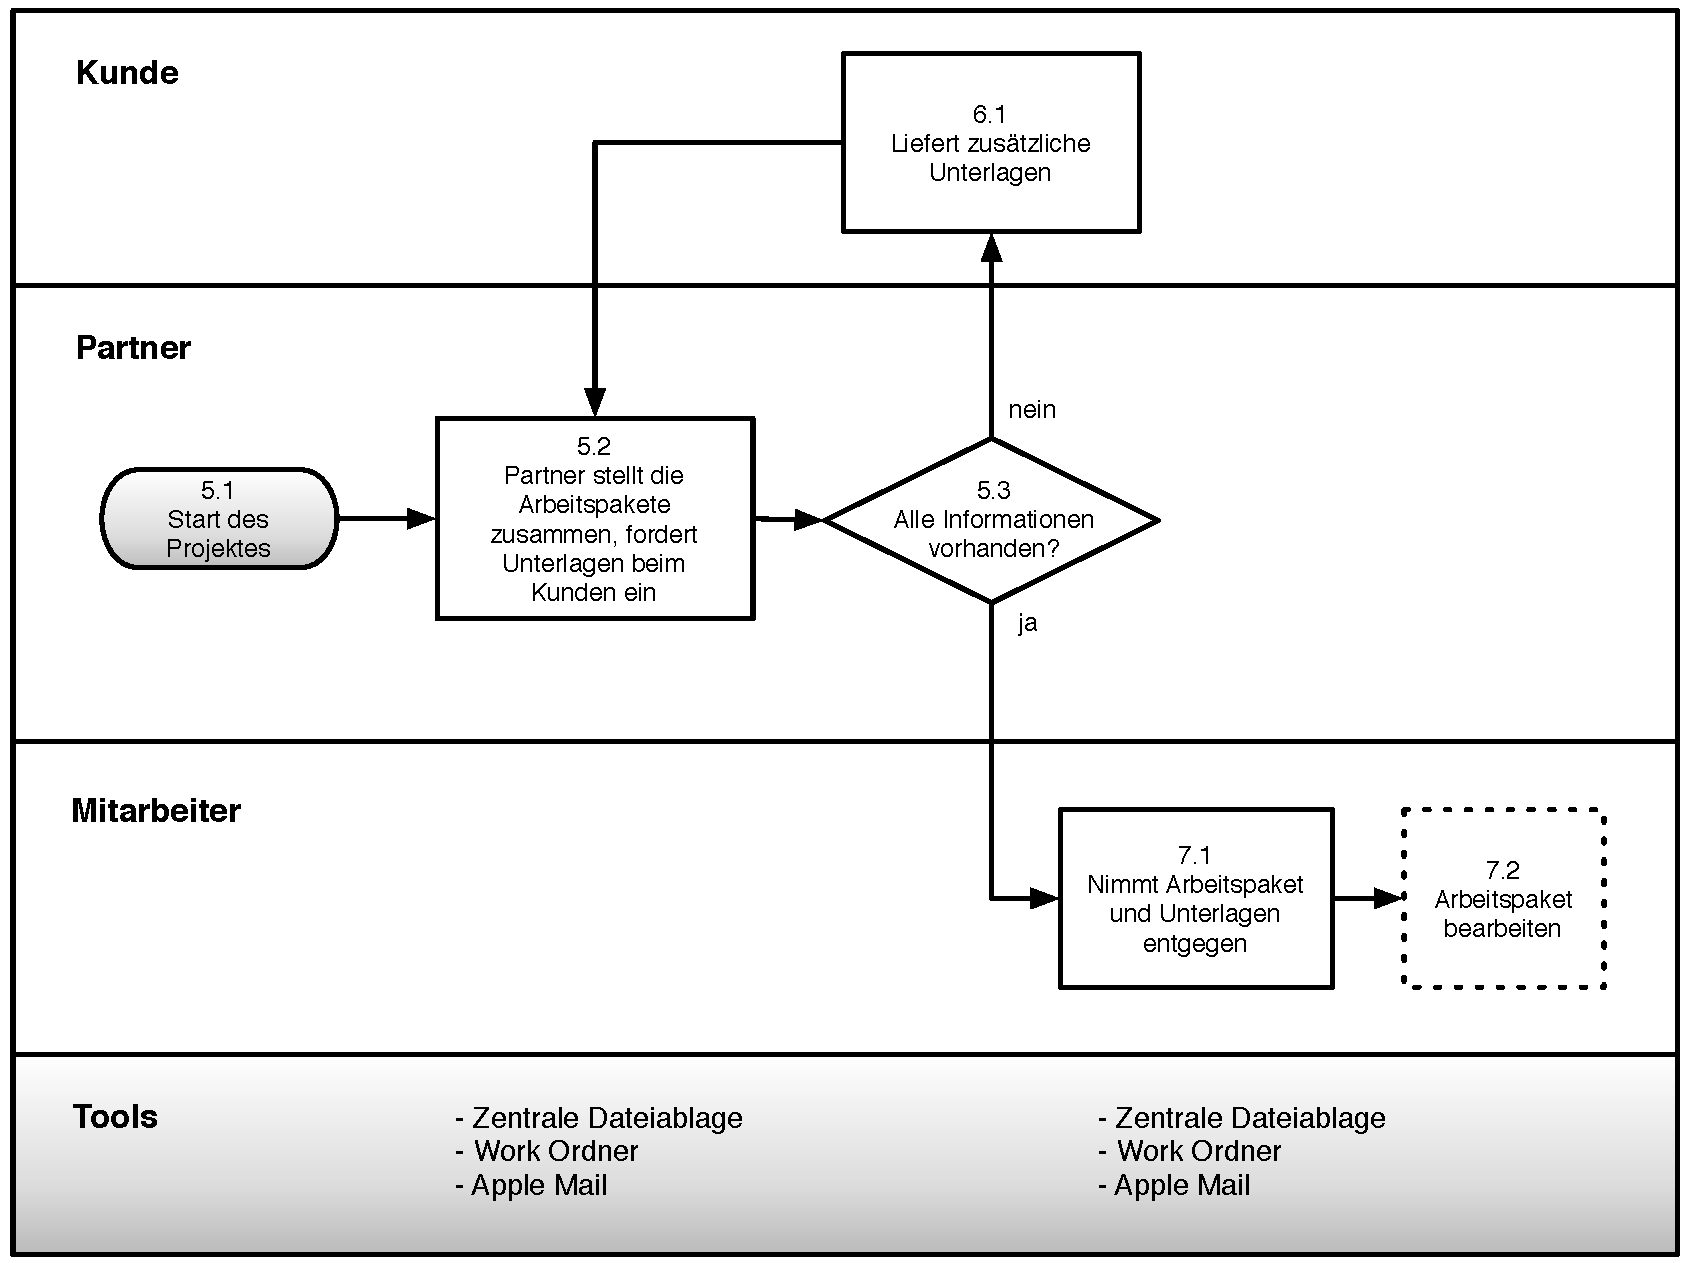
\includegraphics[width=0.99\textwidth,angle=0]{./bilder/analyse/02_ist_prozesse_arbeit_01.pdf}
\caption{Projektumsetzungs Prozess von allink März 2011 1/2}
\label{pic:02_ist_prozesse_arbeit_01}
\end{center}
\end{figure}

Der Partner verschafft sich einen überblick über das Projekt und gruppiert
die zu erledigenden Arbeiten in Arbeitspakete (\textbf{5.2}). Er besorgt alle nötigen Informationen
und Unterlagen, die zur Bewältigung eines Arbeitspaketes notwendig und fordert
bei Kunden wenn nötig noch mehr Informationen und Unterlagen ein (\textbf{6.1}).
Sind alle Informationen vorhanden (\textbf{5.3}) übergibt er das Arbeitspaket.
sie einem Mitarbeiter zur Erledigung.

Der Mitarbeiter nimmt dann das Arbeitspaket entgegen (\textbf{7.1}) und beginnt
mit dessen Bearbeitung (\textbf{7.2}). Stellt sich heraus, dass er sein Arbeitspaket
noch nicht abschliessen kann (\textbf{7.3}) und noch mehr Informationen oder
Unterlagen benötigt (\textbf{8.1}), kommt es oft vor, dass der Mitarbeiter
eigenständig beim Kunden zusätzliche Unterlagen einfordert (\textbf{9.1}).
Sobald er ein Paket abschliessen kann, stellt er alles Erarbeitete zusammen (\textbf{10.1})
und übergibt es dem zuständigen Partner.
Dieser nimmt alle Arbeitspakete entgegen (\textbf{10.2})
und überprüft diese (\textbf{10.3}). Sofern zusätzliche Arbeiten nötig sind,
stellt er diese wieder zusammen und der Bearbeitungsprozess beginnt von neuem (\textbf{5.2}).

\begin{figure}[htbp]
\begin{center}
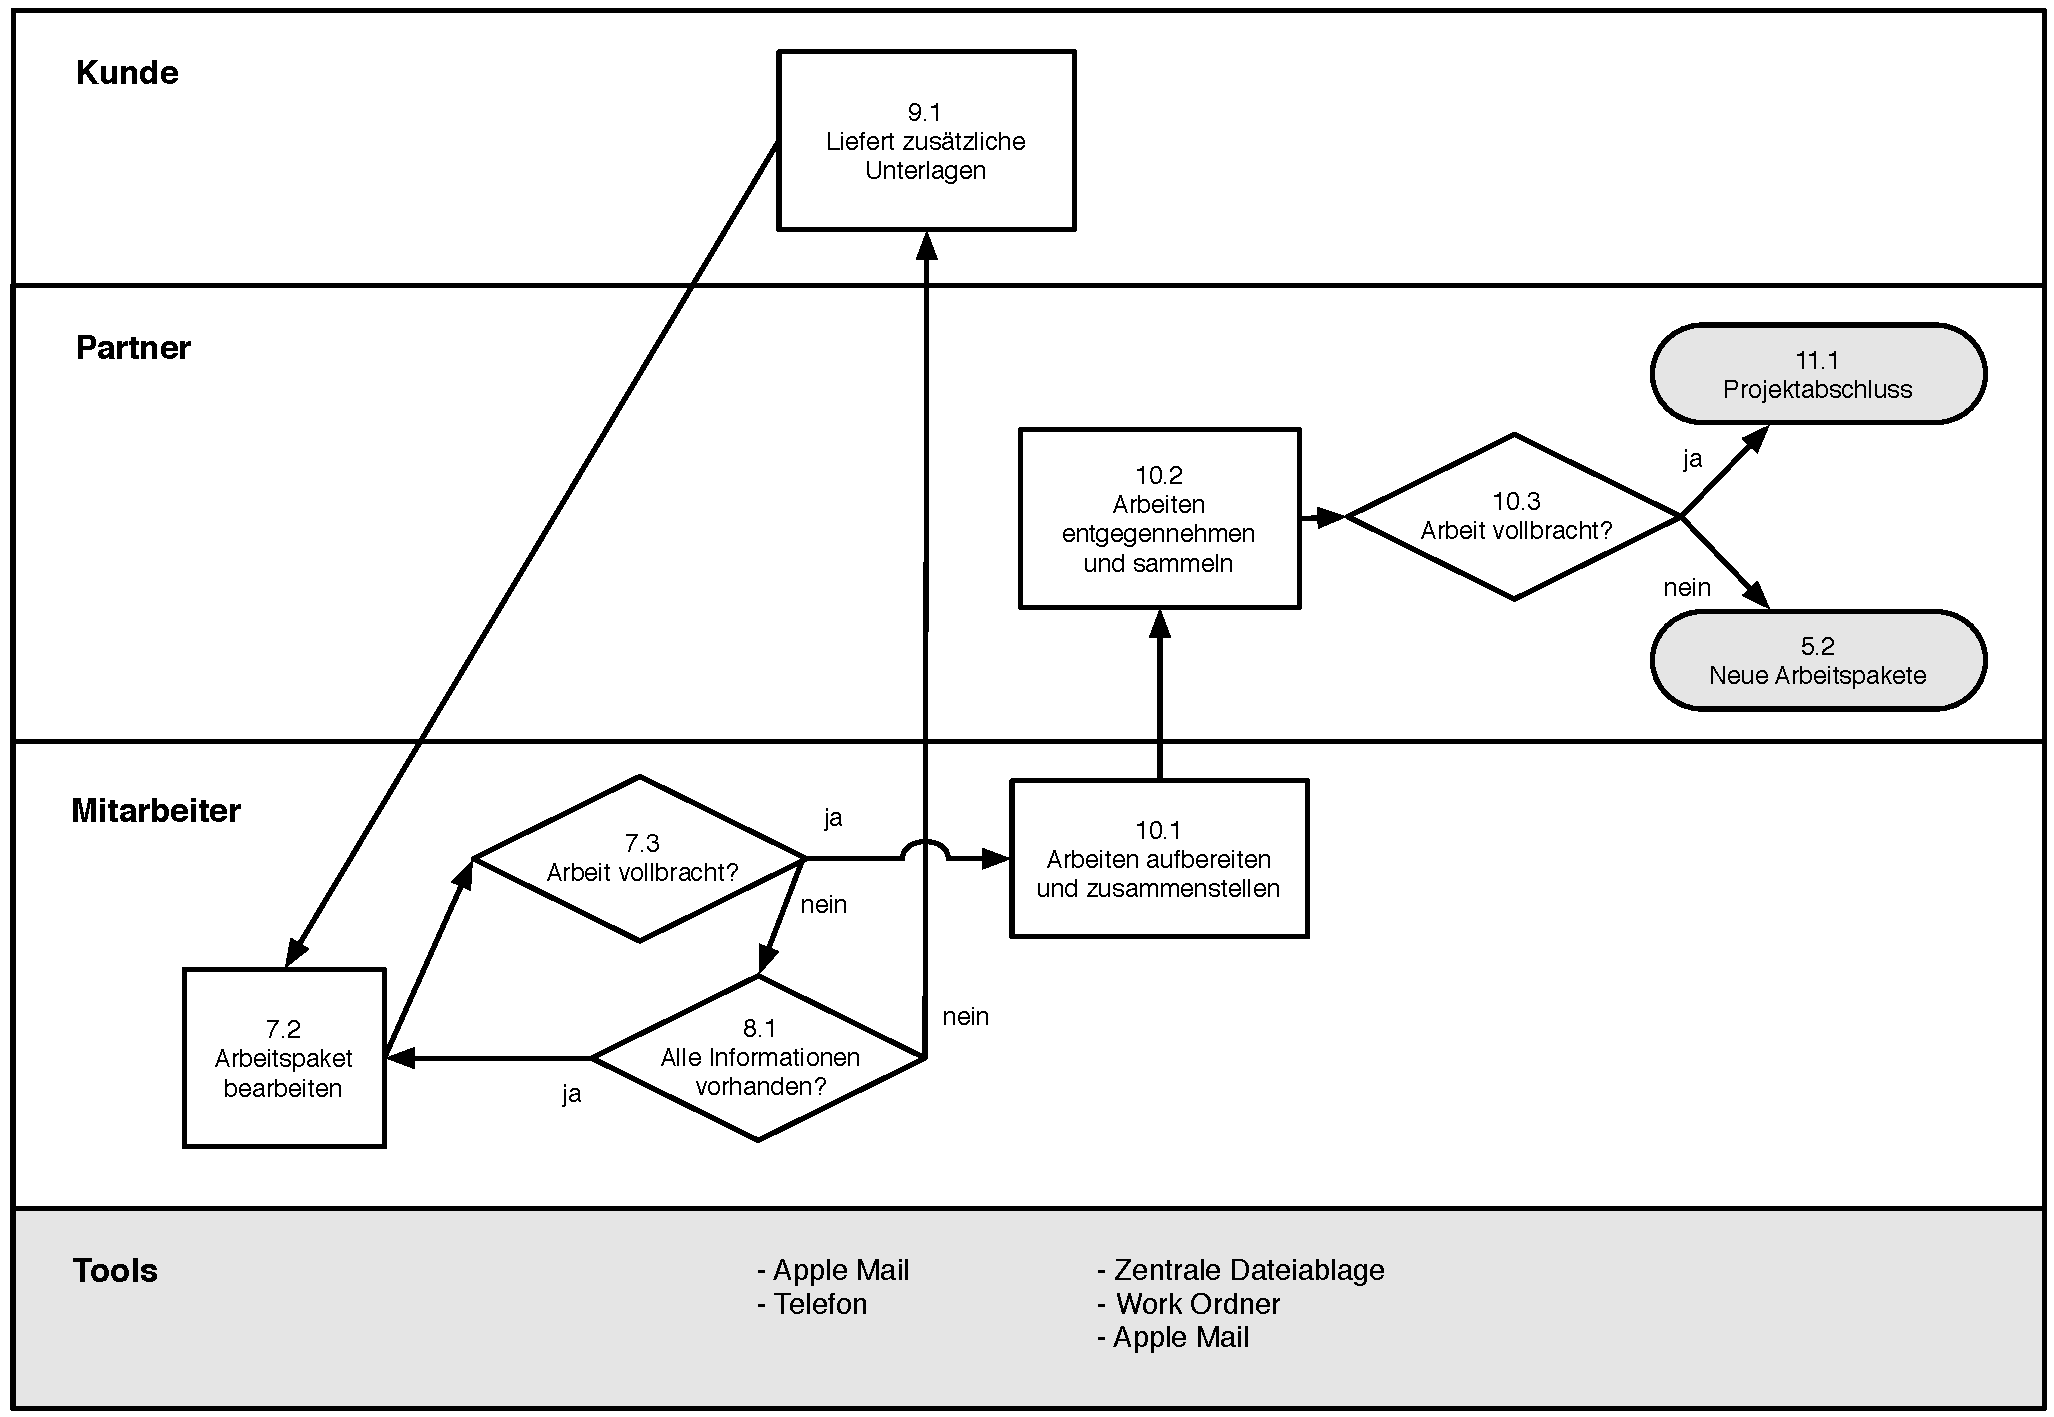
\includegraphics[width=0.99\textwidth,angle=0]{./bilder/analyse/02_ist_prozesse_arbeit_02.pdf}
\caption{Projektumsetzungs Prozess von allink März 2011 2/2}
\label{pic:02_ist_prozesse_arbeit_02}
\end{center}
\end{figure}

Sind alle Arbeiten vollbracht, geht es über in den Projektabschluss (\textbf{11.1}). Dies wirkt
bisschen früh, da der Kunde bis zu diesem Zeitpunkt noch keine Ergebnisse gesehen
hat. Ich habe aber absichtlich die Präsentation der Resultate und das Feedback
des Kunden in den Projektabschluss rein genommen, da ich die Bearbeitung als eigenen
Prozess gekapselt haben möchte. Geht man vom optimalsten Fall aus, kann das
Projekt zu diesem Zeitpunkt wirklich schon abgeschlossen werden. In der Praxis
ist das vor allem bei kleineren Projekten der Fall, wie der Erstellung eines
neuen Flyers, bei dem sich das Konzept über Monate nicht geändert hat und nur
Textkorrekturen und leichte visuelle Anpassungen notwendig sind.

\clearpage

\subsection{Projektabschluss}
Einleitungstext...

\begin{figure}[htbp]
\begin{center}
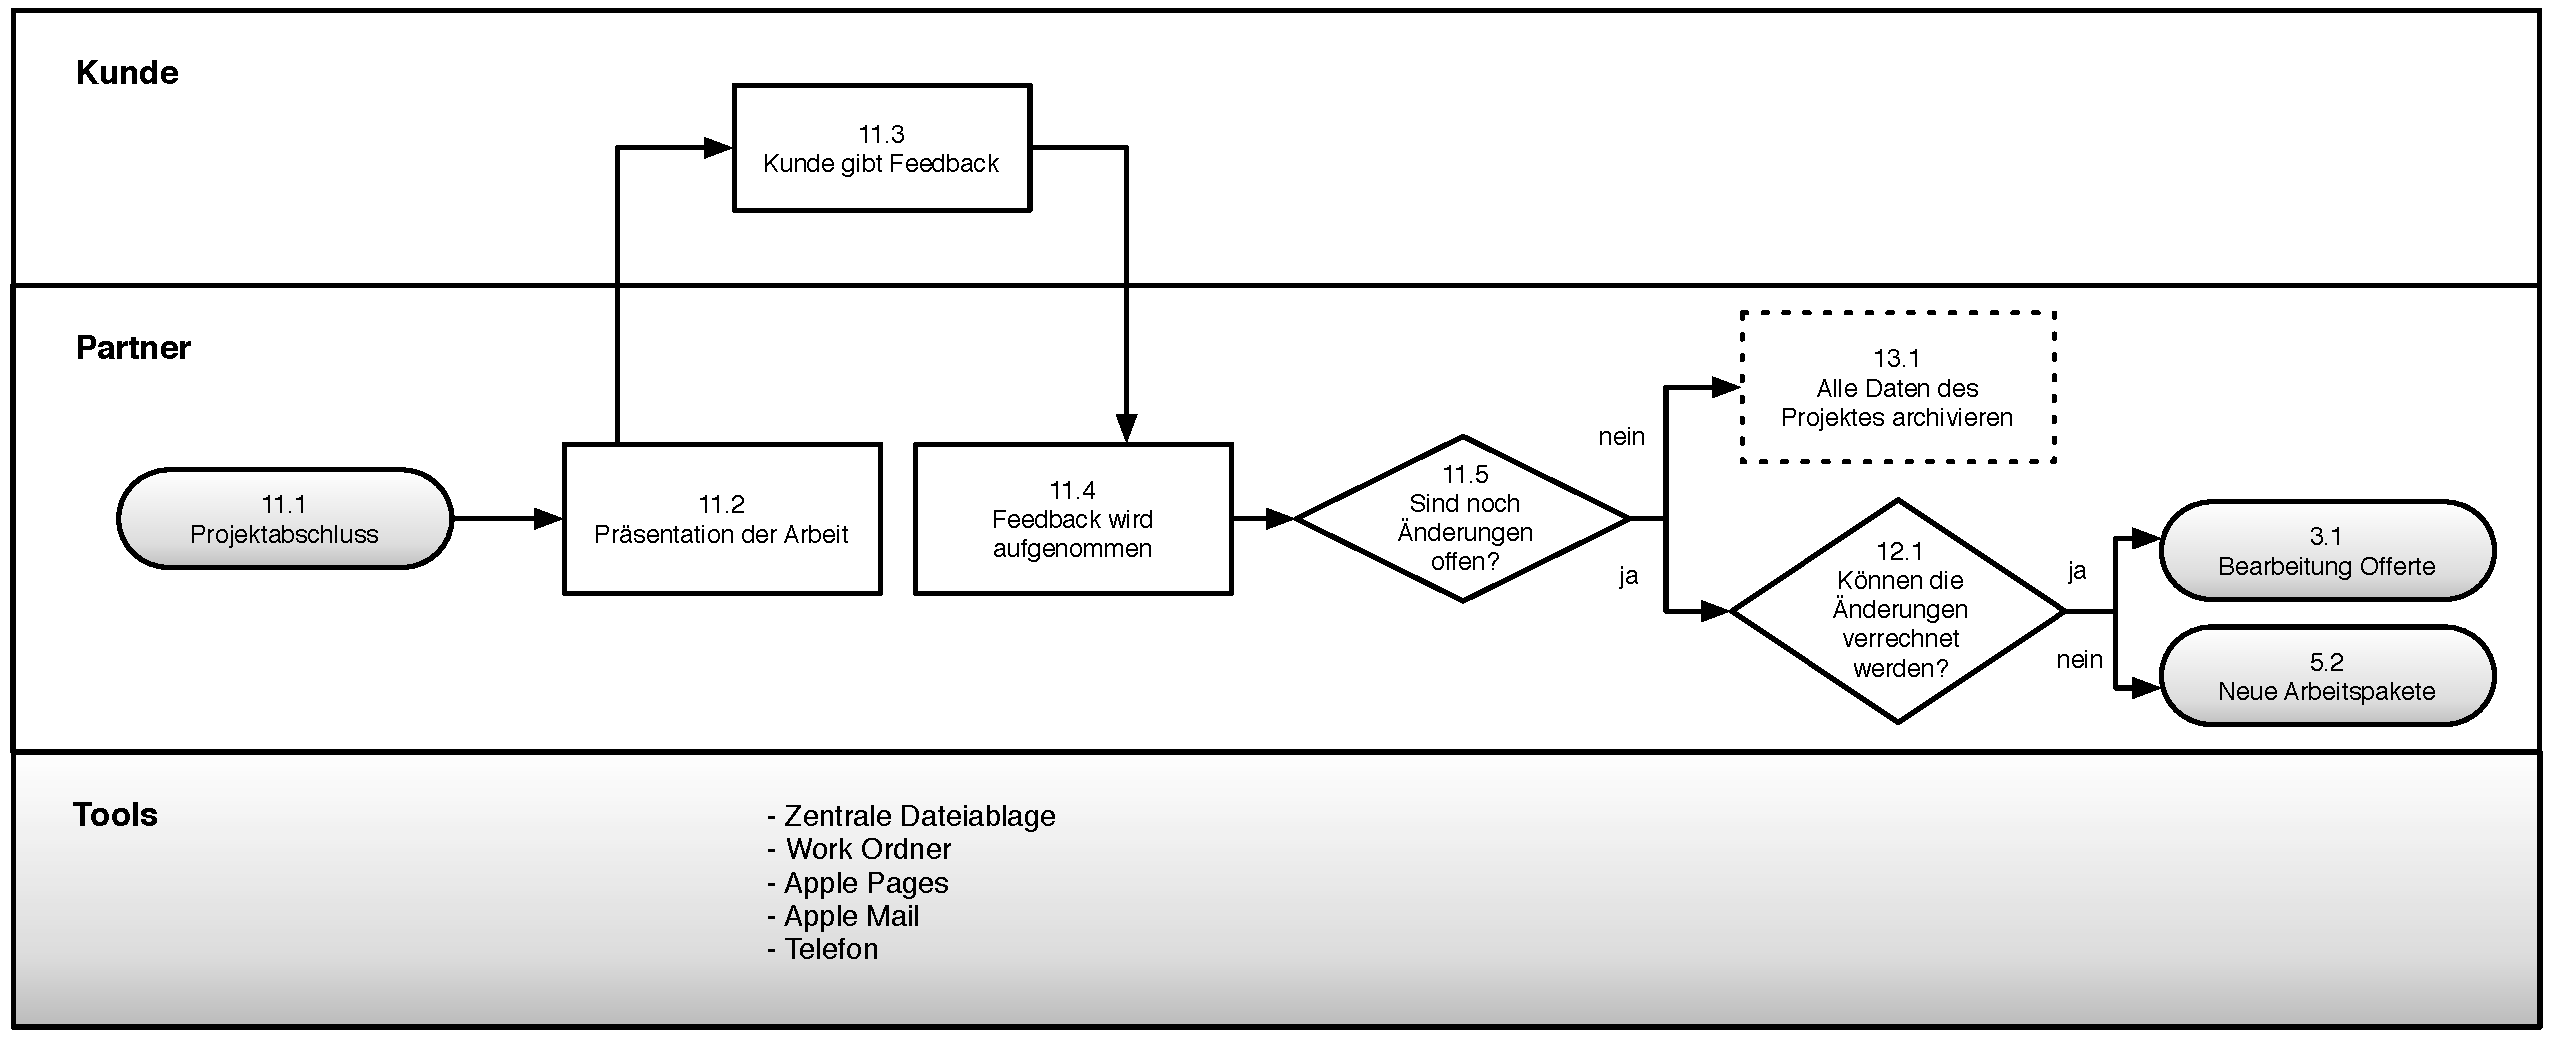
\includegraphics[width=0.99\textwidth,angle=0]{./bilder/analyse/03_ist_prozesse_abschluss_01.pdf}
\caption{Projektabschluss Prozess von allink März 2011 1/2}
\label{pic:03_ist_prozesse_abschluss_01}
\end{center}
\end{figure}

\begin{figure}[htbp]
\begin{center}
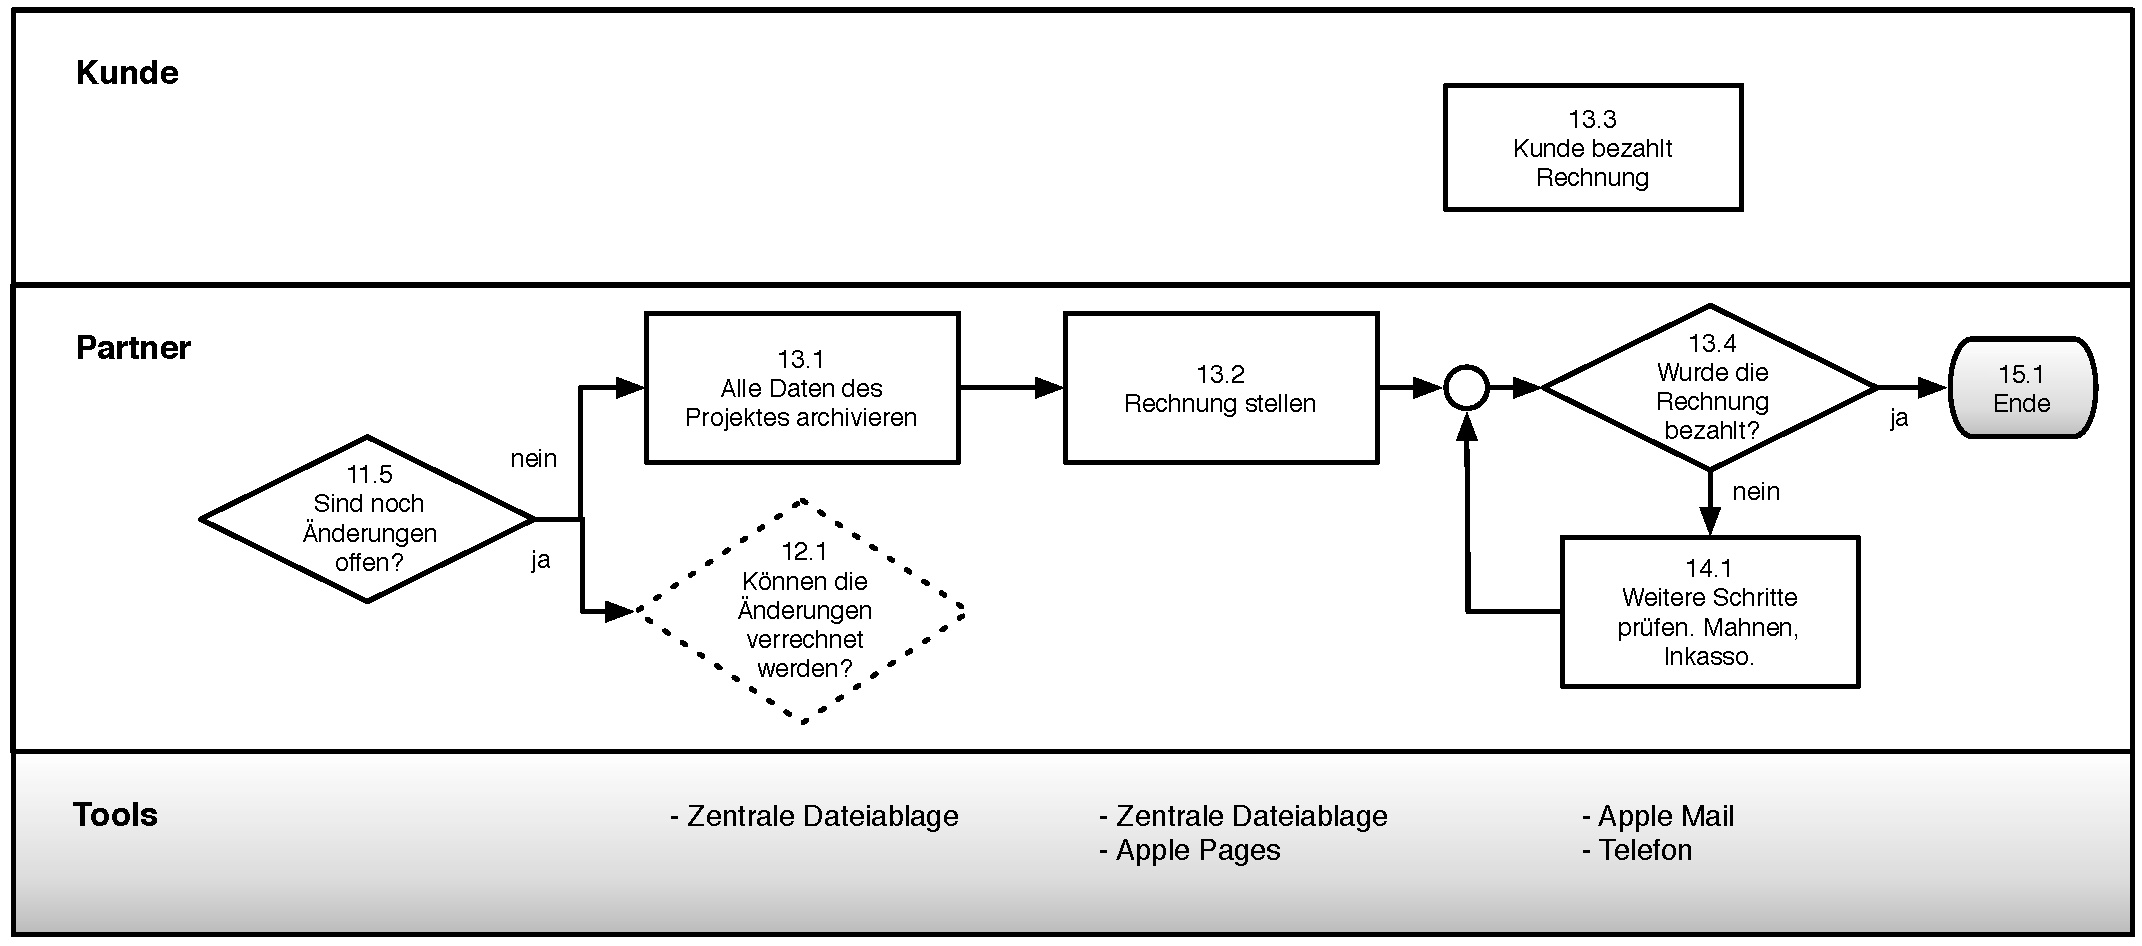
\includegraphics[width=0.99\textwidth,angle=0]{./bilder/analyse/03_ist_prozesse_abschluss_02.pdf}
\caption{Projektabschluss Prozess von allink März 2011 2/2}
\label{pic:03_ist_prozesse_abschluss_02}
\end{center}
\end{figure}

Detaillierte Beschreibung des Prozesses...

\subsection{Verwendete Software}
Bei der Untersuchung der zur Zeit eingesetzten Sofware beschränke ich mich auf jene,
die einen direkten Einfluss auf den aktuellen Projektablauf bei allink haben.
Ich liste keine Software auf, die zur Erbringung der eigentlichen Dienstleistungen
von allink eingesetzt werden.

\begin{figure}[htbp]
\begin{center}
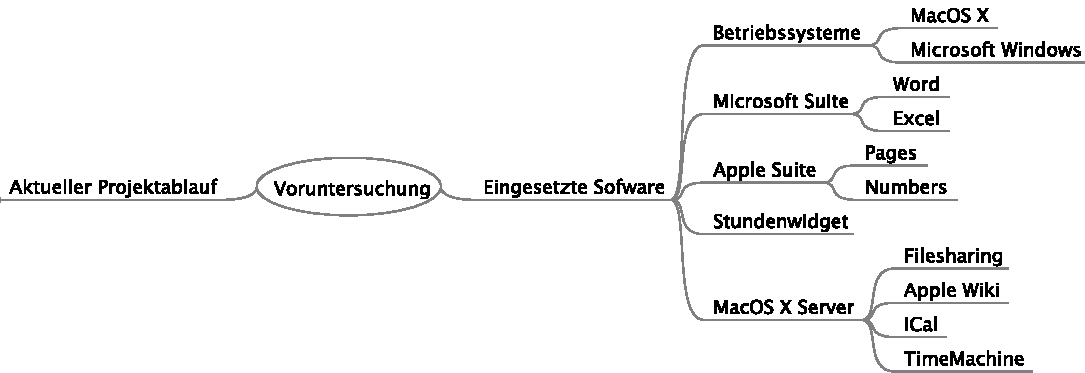
\includegraphics[width=0.95\textwidth,angle=0]{./bilder/analyse/mindmaps/voruntersuchung_software.pdf}
\caption{MindMap Voruntersuchung der eingesetzten Software}
\label{pic:voruntersuchung_software}
\end{center}
\end{figure}

\subsubsection{Betriebssysteme}
Als Hauptbetriebssystem verwendet allink Mac OS X\footnote{Betriebssystem von Apple, \url{http://www.apple.com/macosx/}}.
Es läuft auf allen Arbeitsstationen der Mitarbeiter und Partner. Zusätzlich haben einige der
Entwickler noch Microsoft Windows\footnote{Betriebssystem von Microsof, \url{http://www.microsoft.com/windows/}}
über eine Virtualisierungslösung installiert. Dies wird zu Testzwecken benötigt.

\subsubsection{Microsoft Suite}
Da viele Kunden mit Microsoft Produkten arbeiten benötigt auch allink die
Office Suite\footnote{Microsoft Office für Mac, \url{http://www.microsoft.com/germany/mac}}, 
um Dateien mit Kunden ohne Interoperabilitätsprobleme
austauschen zu können. Nicht jede Arbeitsstation verfügt zur Zeit über eine
Installation.

\subsubsection{Apple Suite}
Für interne Zwecke setzt allink zur Zeit auf die Apple eigene Office Suite
iWork\footnote{Office Suite von Apple, \url{http://www.apple.com/de/iwork/}}.
Pages wird zur Erstellung von Offerten und Rechnungen verwendet. Mit Numbers
werden Tabellenkalkulationen wie die Liquiditätsplanung oder Lohnblätter erstellt.
Da dies aber lange nicht so von der Geschäftsleitung kommuniziert wurde, existieren
auch einige Excel Files, das Pendant der Microsoft Office Suite.

\subsubsection{Stundenwidget}
Das Stundenwidget ist eine selbst geschriebene Software von allink und läuft
im Dashboard\footnote{Widget Lösung von Apple, \url{http://www.apple.com/downloads/dashboard/}} des Betriebssystems.
Es ermöglicht Stunden auf ein Projekt zu buchen, wie man auf dem Screenshot \ref{pic:ist_widget}
sehen kann.

\begin{figure}[htbp]
\begin{center}
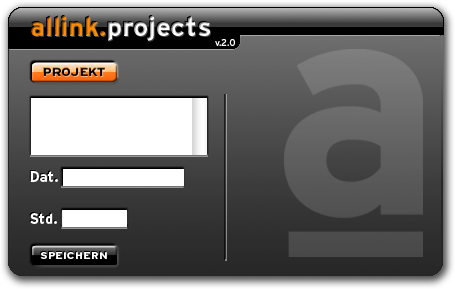
\includegraphics[width=0.55\textwidth,angle=0]{./bilder/analyse/ist_widget.png}
\caption{Aktuelles Stundenwidget von allink}
\label{pic:ist_widget}
\end{center}
\end{figure}

Die Daten werden auf dem
eigenen Server gespeichert und pro Projekt abgelegt. Dieses Widget ist auf allen
Arbeitsstationen installiert und wird von den Mitarbeitern gelegentlich verwendet
um ihre Stunden auf ein Projekt zu rapportieren.

\subsubsection{MacOS X Server}
Auf dem Server liegt das zentrale Dateiablagesystem. Die Zugriffsrechte können
auf dem Server für jede Freigabe definiert werden. So haben zum Beispiel
die Mitarbeiter keinen Zugriff auf den Administrationsordner der Geschäftsleitung.
Über diesen Server laufen auch die einzelnen Firmenkalender der Partner. Sie
können so gemeinsam Termine buchen und haben stets Einblick in die anderen
Kalender.